%!TEX encoding = UTF-8 Unicode
%!TEX root = ../paper.tex

\section{Architecture}
\label{sec:architecture}

%Design and Implementation
We introduce Shuttle, an intrusion recovery service for \ac{PaaS}. Our goal is to help \ac{PaaS} tenants to recover from the following problems in their applications:
\begin{itemize}
  \item \textit{Software vulnerabilities:} non-authorized persons compromise the state by exploiting software vulnerabilities that allow requests to be executed. For instance, a hacker does a SQL injection attack, causing the execution of otherwise invalid queries to the database.
  \item \textit{Faulty requests:} users that are somehow authorized compromise the application state accidentally or intentionally issuing valid requests. For example, a hacker steals users' credentials then uses them to access their data.
\end{itemize} 
 
%attack example
%For instance, two common attacks that can be used to compromise application state consist in: (1) attackers stealing valid users' credentials and using them to access their data; and (2) doing a SQL Injection attack by mixing SQL meta-characters with normal input and doing otherwise invalid queries to the database. Both attacks can be performed using apparently valid requests, so many prevention mechanisms fail to block them.

%Summary
Applications supported by Shuttle can operate in one of two phases: \textit{normal execution} and \textit{recovery}. During \emph{normal execution}, Shuttle records the data required to recover the application's state: it does periodic database snapshots, logs  user requests and database accesses. When an intrusion is identified, tenants use Shuttle to recover their applications starting the recovery phase.

The processes described in Section \ref{sec:background} lead us to define \textit{how to remove intrusion effects} and \textit{how to recover a consistent state}. During the \emph{recovery phase}, Shuttle removes  intrusion effects creating a \textit{branch} of the system execution in which it loads a snapshot, which contains the application state before the intrusion began. It builds a consistent state by replaying (re-executing) in the new branch, the legitimate requests logged during \emph{normal execution}, performing either selective or full replay (Section \ref{sec:recovery}). In the meantime, the incoming requests are executed in the previous branch. When ready, it sets the new branch as the single execution branch.

%PaaS
\ac{PaaS} platforms offer services to build, deploy and manage applications. Shuttle aims to be integrated by CSPs into their \ac{PaaS} platforms as a novel service. 
%Services provided in \ac{PaaS} are expected to be well-tested and available without setup because they are offered by \ac{CSP} and shared by multiple tenants.
We assume a minimal \ac{PaaS} architecture to let Shuttle as generic as possible. We consider a client-server model in which clients access applications using the HTTP protocol\footnote{Shuttle also supports HTTPS by ending the connections at the proxy.}. HTTP requests are received by a load balancer that forwards them to web/application servers, which access a shared database. {PaaS} components are represented with solid line in Figure \ref{fig:shuttle_architecture}, while Shuttle components are represented with dashed line. The components of a \ac{PaaS} platform with Shuttle are:

\begin{itemize}
  \item \textit{Proxy:} Logs every HTTP user request, adds a new field to its header, and forwards it to the load balancer. The proxy functionality might be part of the load balancer but conceptually it is a different component.% and currently it is also implemented separately.
  \item \textit{Load balancer:} Routes requests to different application servers taking into account their load (part of the \ac{PaaS} platform).
  \item \textit{Application servers:} The application (or web) servers are the components of the \ac{PaaS} platform that run the application logic. This logic uses a library to access the database service. Shuttle uses a \textit{database client interceptor} mechanism in this library to log the data items accessed per request.
  \item \textit{Database instances:} A set of database servers used to store the application persistent state. Shuttle includes in each instance  a \textit{database proxy} that logs the requests that accessed each data item and determines the dependencies between requests.
  \item \textit{Shuttle storage:} A scalable storage component that stores requests, responses and metadata.
  \item \textit{Manager:} Retrieves dependencies and coordinates the recovery process. 
  \item \textit{Replay instances:} A set of instances with HTTP clients that read previously executed requests from the Shuttle storage and invoke the application servers to re-execute the requests during the recovery process. These worker instances are coordinated by the manager.
\end{itemize}

\begin{figure}
  \centering
  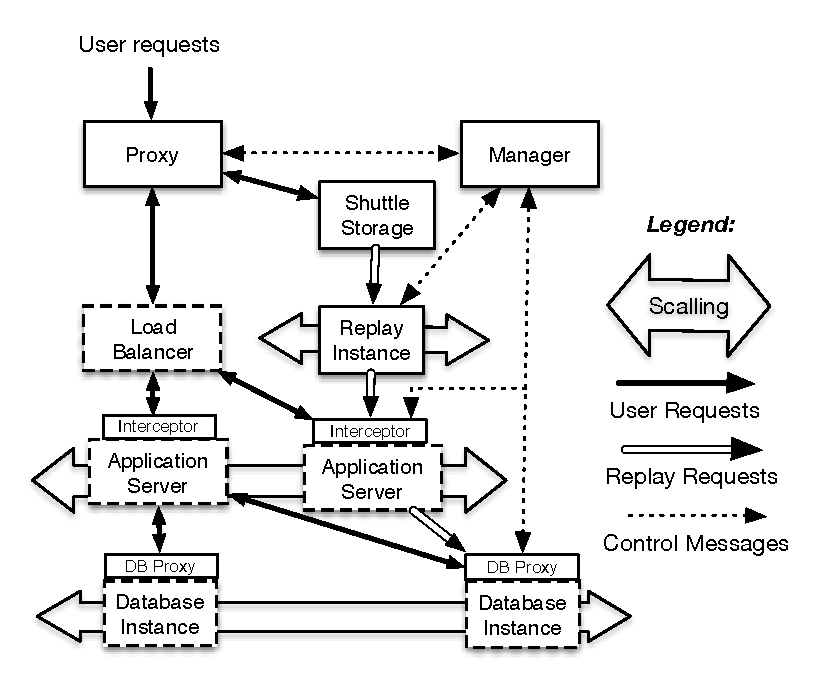
\includegraphics[width=0.8\columnwidth]{images/architectureTiers}
  \caption{Shuttle architecture (dashed components are original from \ac{PaaS}). %The proxy logs the user requests into the Shuttle storage. The manager coordinates the recovery process where the replay instances replay the user requests.
  }
  \label{fig:shuttle_architecture}
\end{figure}

%Why Paas?
PaaS offerings are supported by a computing infrastructure, often provided as a service (IaaS model), able to scale the application allocating new instances on-demand or automatically, to maintain the quality of service despite demand oscillations. This elasticity  allows to allocate replay instances and to scale the application to attend the requests issued by them during the recovery process.
With the pay-per-usage model, these resources become a cost only when there is a recovery. The remaining cost of the service comes from storing client requests and database snapshots. Our design aims to optimize the available resources to reduce the recovery period and costs. 


%Database
Unlike previous works, our design encompasses distributed databases. We assume without loss of generality that applications store their state in distributed key-value stores, such as Dynamo \cite{Decandia2007}, where the values are accessed using a \acf{CRUD} API. This simple API reduces the performance overhead to track accesses while the independence between keys turns Shuttle into a scalable service. Shuttle can be extended to support other NoSQL stores.

%the storage
The \emph{Shuttle storage} keeps the content of the user requests and responses. Although we do not consider this aspect in the architecture, this store can be replicated to a remote site to allow tolerating catastrophic failures in a datacenter.

We consider the Shuttle components to be part of the trusted computing base since their integrity and availability are critical to recover the application. We assume that intrusions tamper the application data, which is stored in the database.





%%%%%%%%%%%%%%%%%%%%%%%%%%%%%%%%%%%%%%%%%%%%%%%%%%%%%%%%%%%%%%%%%%%%%%%%%%%%%%%%%%%%%%%%%%%%%%%%%%%%%%%%%%%%%%%%%%%%%%%%
\section{Normal Execution}
\label{sec:architecture:normal_execution}

Shuttle logs the data it needs to recover applications during the normal execution phase: user HTTP requests, application HTTP responses, database items accessed by each request and sequence of operations to each database item (Figure \ref{fig:normal_execution}). In this section, we describe the normal execution phase following the path that a request takes to be processed.

\begin{figure}
  \centering
  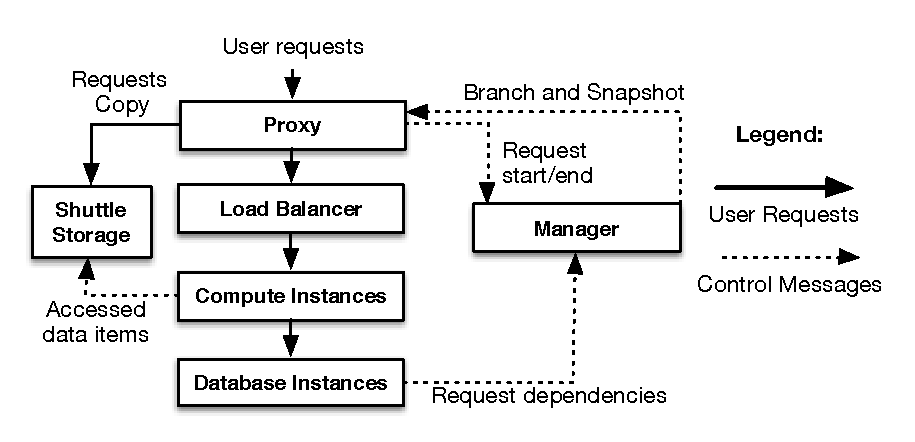
\includegraphics[width=0.7\linewidth]{images/normalExecution}
  \caption{Interaction between components during normal execution.}
  \label{fig:normal_execution}
\end{figure}


\subsection{Proxy}
\label{sec:architecture:proxy}

%O proxy coloca o timestamp e guarda os pedidos
The proxy intercepts all user HTTP requests, except those to static contents (e.g., images), and adds a new header field named \acf{SRD}. \ac{SRD} contains a few subfields: \acf{RID}, an unique timestamp; \emph{branch} and \emph{snapshot} that define the database branch and snapshot of the request (Section \ref{sec:architecture:snapshot}); a \emph{restraint flag} used to support runtime recovery (Section \ref{sec:recovery:runtime_recovery}). 

The proxy also intercepts every application response, associates the response with the original request and adds a new timestamp to track the ending of the request execution. Requests, responses and their timestamps are stored in the \emph{Shuttle Storage} using asynchronous I/O, which permits the operations to proceed before the transmission has finished. 


%%%%%%%%%%%%%%%%%%%%%%%%%%%%%%%%%%%%%%%%%%%%%%%%%%%%%%%%%%%%%%%%%%%%%%%%%%%%%%%%%%%%%%%%%%%%%%%%%%%%%%%%%%%%%%%%%%%%%%%%
\subsection{Application server and database instances}
\label{sec:architecture:database}

%Access tracking at server and database sides
In order to associate every database operation with the \ac{SRD} of the source HTTP request, we propose to modify the application server adding it an \emph{interceptor}. This component is invoked by the database client library before and after the request processing: before, the interceptor gets the \ac{SRD} and logs the accessed data items; after, it stores the log of accessed data items in the \emph{Shuttle Storage}. This avoids having to modify the tenants' applications.
%mpc: modifiquei bastante; verificar

%Tracking operarations
Every database operation involves calling the \emph{database proxy}. The proxy logs the operation's \ac{RID} and type (put, get, delete) and uses its \emph{branch} and \emph{snapshot} subfields to select the correct data item version. The sequence of operations to a data item defines its \emph{operation list}.  
The access order is ensured by a read-write lock that serializes the access to the value of the data item allowing multiple reads but only a single write concurrently. This pessimistic concurrency control may decrease the system performance in comparison with a multi-version concurrency control scheme, in which the \ac{RID} would be written among the value and parsed during the read operation. Nevertheless, we used this form of concurrency control for the sake of simplicity.
%
The \emph{operation list} and lock of each data item are stored in a Hash Table that supports concurrent accesses.

Periodically, each database instance iterates the operation list of every data item to establish the dependencies between requests. The manager retrieves, asynchronously, the start and end timestamps of each request, collected by the proxy, and its dependencies, collected by the database instances, to generate the dependency graph (Section \ref{sec:recovery:dependencies}).

\subsection{Snapshot}
\label{sec:architecture:snapshot}

A \emph{snapshot} is a set of versions of every data item in the database. Our service loads a snapshot to remove the intrusion effects and replays the later requests to recover an updated application state. 

Performing snapshots in distributed key-value NoSQL databases like Dynamo is not trivial since snapshots have to be consistent with the user requests. We consider each user request may include multiple database accesses, each of them to multiple database servers, without using transactions. 
If Shuttle replays a request on a snapshot that contains part of the persistent state written by a request during its first execution, the replay will be inconsistent. Therefore each snapshot shall be \emph{global request-consistent} containing either all or none of the database updates made by every request \cite{checkpoint-survey}. 

The snapshot shall be non-blocking: applications shall not stop their execution while taking snapshots. For instance, a straightforward way to take a request-consistent global snapshot is to stop processing new requests, waiting until the currently executing requests finish, and then making a copy of each data item. However, this solution causes application downtime.

%Our solution
Our solution leverages the existence of a single load balancer and, consequently, a single proxy that adds the \ac{SRD} field to every request. Every \ac{SRD} contains a \ac{RID} (the instant when the request is retrieved). In order to create a snapshot, tenants define a future instant in time $t$ when the snapshot will occur. The instant, named \acf{SID}, identifies the snapshot. The manager passes the \ac{SID} to every database proxy.

Database proxies use the \ac{SID} to define the version of the data item used by the operations. Operations with \acf{RID} lower than the scheduled snapshot instant (\ac{RID} $<$ \ac{SID}) access the version before the snapshot. Otherwise, the operations access the latest data item version. This mechanism splits requests to accomplish a request-consistent global snapshot, and allows tenants to schedule snapshots without application downtime. 

We avoid blocking the application to copy the versions using a copy-on-write and incremental method: a new version is created only when the data is written for the first time in each snapshot. Since a data item may not be written in every snapshot, we associate a \emph{version list} to every data item. This list tracks in which snapshots the data item has been written. \hl{Shuttle provides such capability to any key-value database by using the concatenation of the key with the \ac{SID} as key to store the data. Checkpoints are stored locally and may be replicated to a remote site.}

A snapshot might become inconsistent if a request with \ac{RID} greater than the snapshot instant \ac{SID} reads a version belonging to the snapshot \ac{SID} and a concurrent request with \ac{RID} lower than \ac{SID} overwritten that version. Storing a new version and adding a flag on the version list solves the problem. Nevertheless, we expect this to happen only in rare occasions.




